\RequirePackage{ifpdf}
\ifpdf
	\documentclass[11pt,oneside,a4paper,pdftex]{article}   %two-page printing
\else
	\documentclass[11pt,twoside,a4paper,dvips]{article}   %two-page printing
\fi

%\documentclass[a4paper, 12pt]{article}
\addtolength{\hoffset}{-1.9cm}
\addtolength{\voffset}{-1.9cm}
\addtolength{\textwidth}{+3.8cm}
\addtolength{\textheight}{+3.8cm}
\usepackage[latin1,utf8]{inputenc}
\usepackage[czech]{babel}
\usepackage{icomma} % ceska desetinna carka
\usepackage{csquotes}
\usepackage{listings}
\usepackage{amsmath}
\usepackage{amsthm}
\usepackage{amsfonts}
\usepackage{mathrsfs}
%\usepackage[T1]{fontenc}
\ifpdf
	\usepackage[pdftex]{graphicx} % dvips or pdftex
\else
	\usepackage[dvips]{graphicx} % dvips or pdftex
\fi
\usepackage[center]{subfigure}
\usepackage{amsfonts}
\usepackage[dvips]{color}               %for using colors
%\usepackage{showframe}                 %zobrazuje okraje stranky
\usepackage[justification=justified,hang]{caption}
\usepackage{textpos}
\usepackage{url}
%\usepackage{fancybox}
\usepackage{verbatim}
\usepackage{fj}
\ifpdf
	\usepackage[pdftex,unicode,colorlinks]{hyperref}
\else
	\usepackage[unicode]{hyperref}
\fi


%FIXME: odlišit font, aby části kódu byly odlišitelné od okolního textu
\lstset{ %
language=Matlab,           % choose the language of the code
basicstyle=\ttfamily,   % the size of the fonts that are used for the code
numbers=none,             % where to put the line-numbers (none, left, ..)
numberstyle=\scriptsize,  % size of the fonts used for the line-numbers
stepnumber=1,             % step between two line-nums. If "1" each line nmbrd
numbersep=10pt,            % how far the line-numbers are from the code
%backgroundcolor=\color{white},
	% choose the background color. You must add \usepackage{color}
showspaces=false,         % show spaces adding particular underscores
showstringspaces=false,   % underline spaces within strings
showtabs=false,           % show tabs within strings
frame=none,	          % adds a frame around the code (single, none, ...)
tabsize=2,	          % sets default tabsize to 2 spaces
captionpos=b,             % sets the caption-position to bottom
breaklines=false,          % sets automatic line breaking
breakatwhitespace=true,   % sets if automatic breaks should only happen at \s
%escapeinside={\%*}{*)}   % if you want to add a comment within your code
}

\title{1. Zpráva pro předmět 3D Počítačové vidění -- A4M33TDV}
\date{17. 11. 2011}
\author{Filip Jareš, jaresfil@fel.cvut.cz}

\begin{document}

\maketitle

\section{Úvod}

Tato zpráva popisuje semestrální práci pro předmět 3D počítačové vidění. Cílem této semestrální
práce je na základě dvanácti fotografií vybraného objektu (portálu/dveří) zrekonstruovat nasnímanou
scénu a vytvořit trojrozměrný digitální model této scény.


% Notes:
%
% terminology:
%	correspondence = truth,
%	match = algorithm’s result; hypothesised corresp.


\section{Popis metody}

Pokusne citace:
\cite{Hartley2004}
\cite{SaraLectures}

% Použitý fotoaparát: Canon DIGITAL IXUS 80 IS

Nasnímané obrázky

	\begin{figure}[htb]
		\centering
		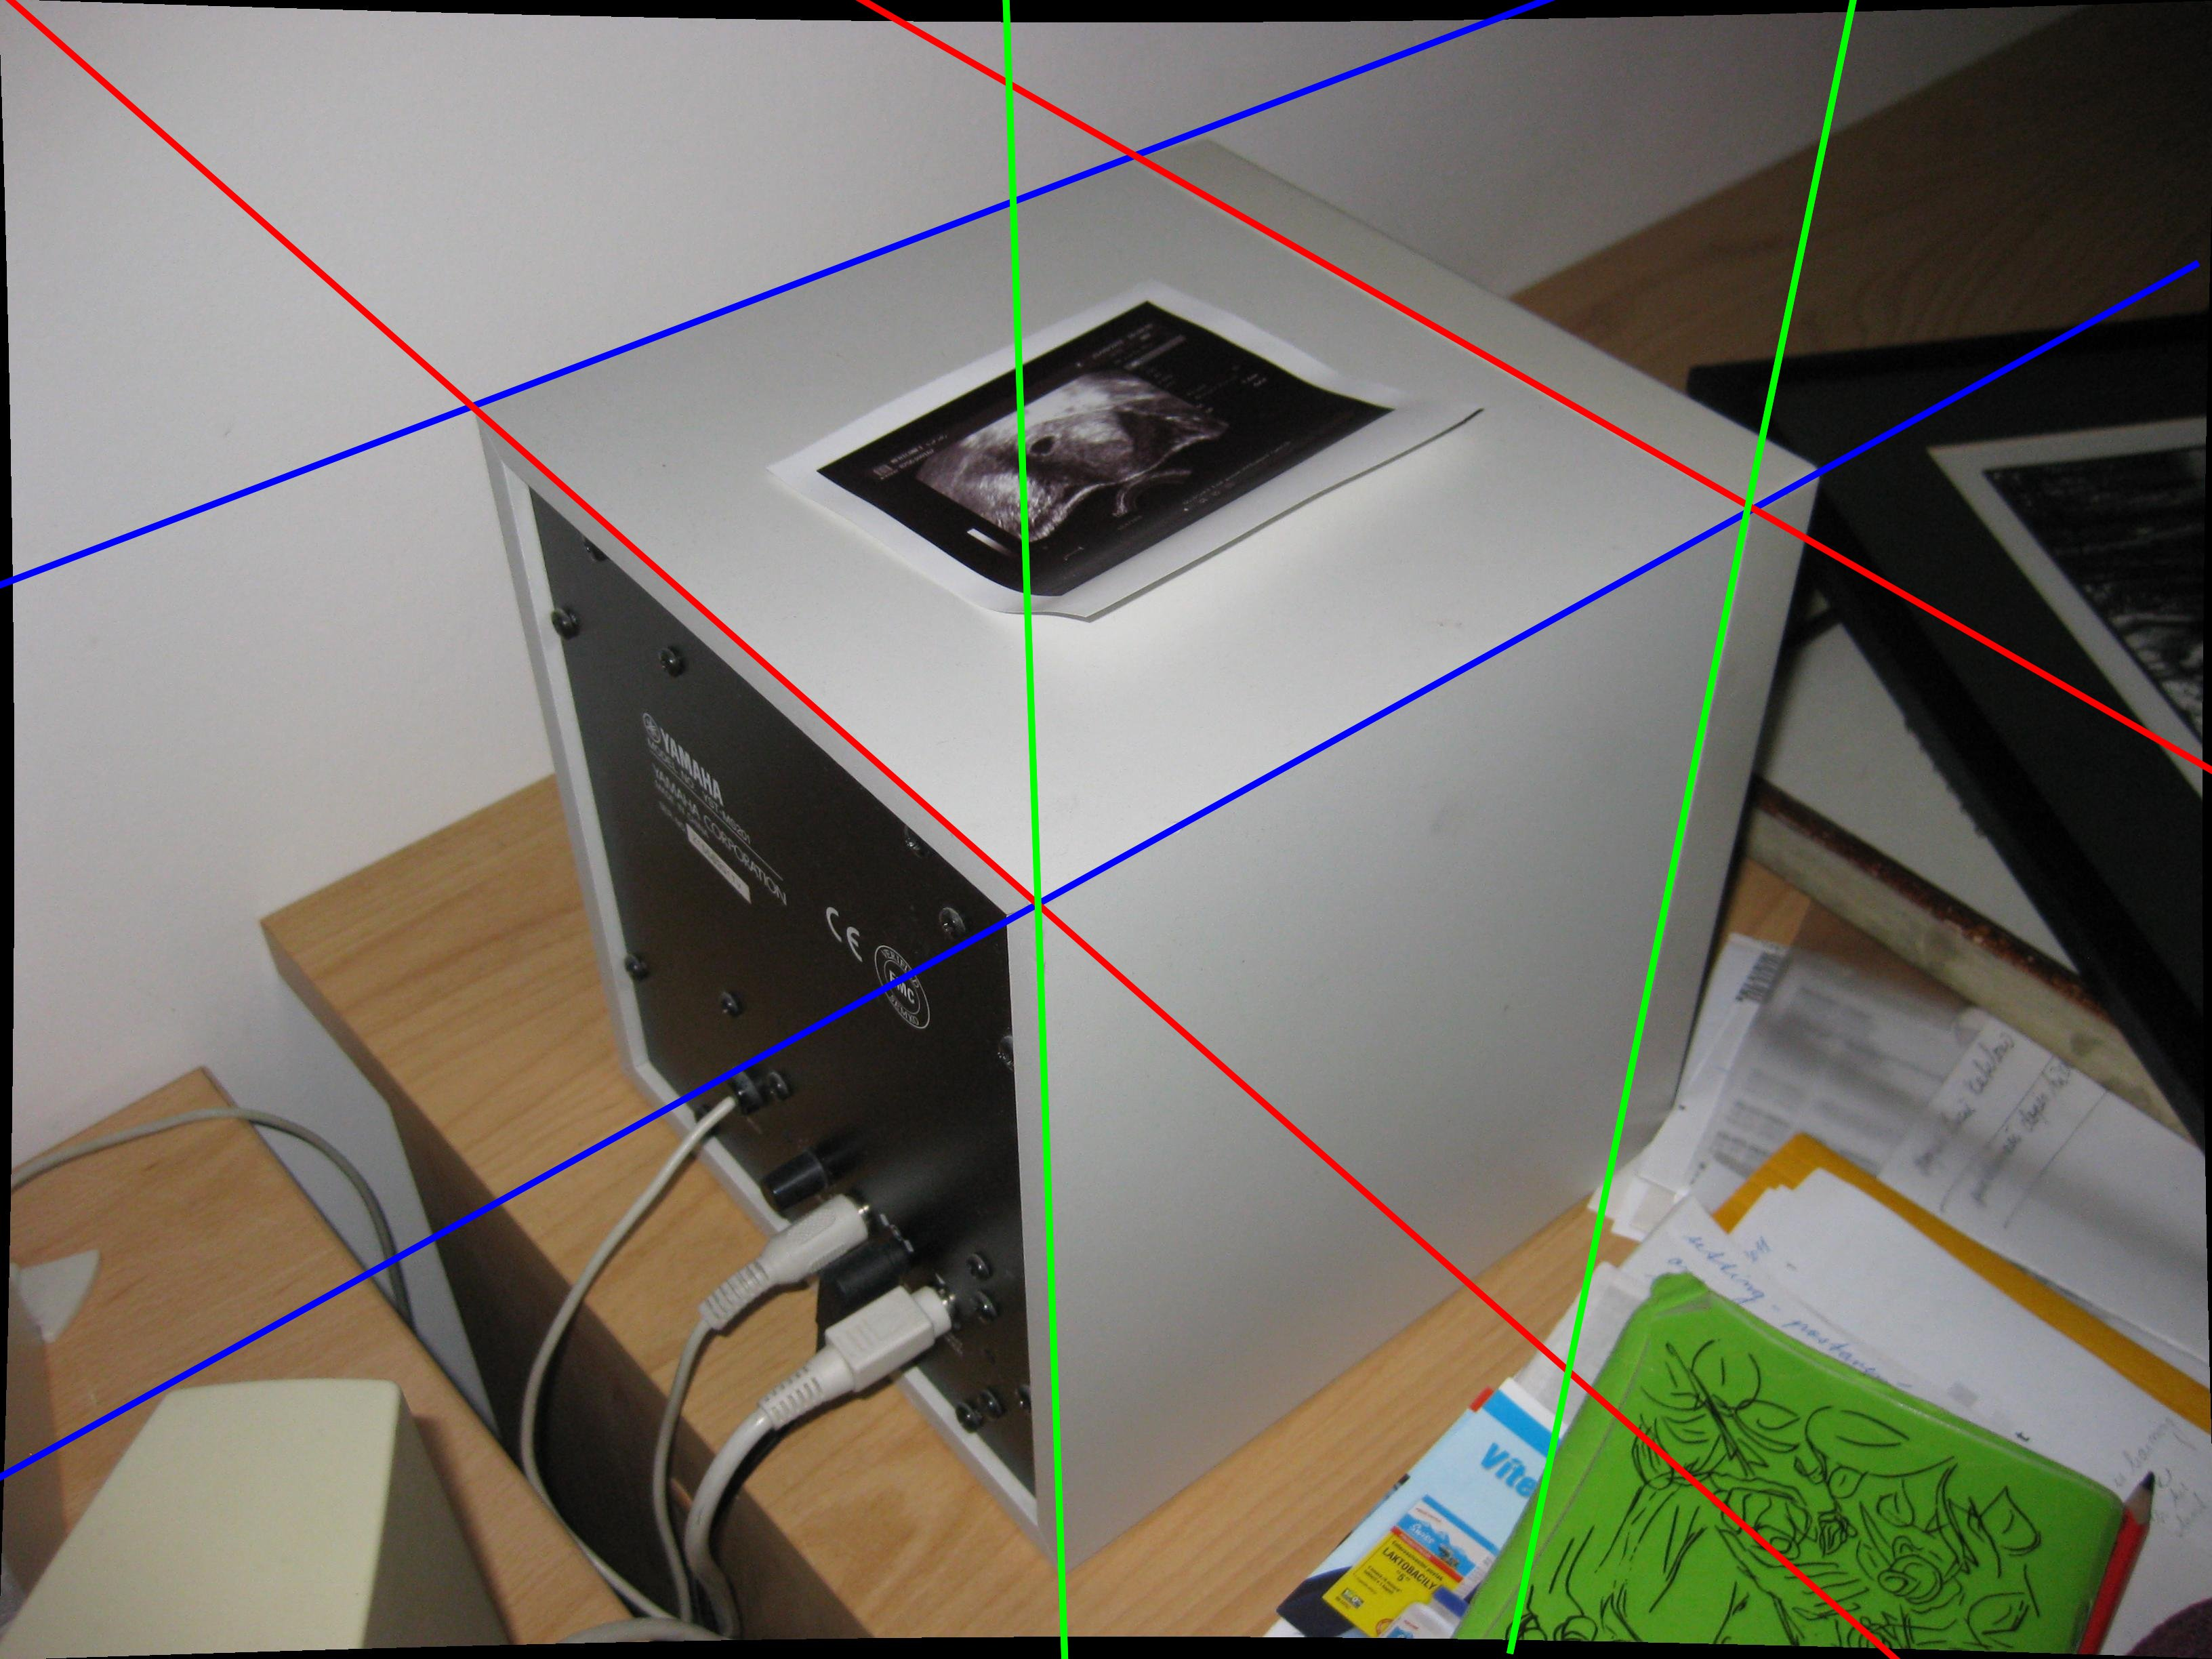
\includegraphics[width=16cm]{pictures/linear/cube.jpg}
		\caption{Snímek pravoúhlého objektu použitého pro kalibraci kamery. Červeně, zeleně
		a modře jsou vyznačeny rovnoběžky ve třech navzájem kolmých směrech, které byly
		použity pro nalezení úběžníků.}
		\label{fig:cube}
	\end{figure}


	\begin{figure}[htb]
		% dummy content, to make the rendering faster while under construction
			\centering
			\subfigure[] {
				\fbox{\begin{minipage}{3cm}\hfill\vspace{4cm}\end{minipage}}
				\label{fig:firstInputImage}
			}
			\subfigure[] {
				\fbox{\begin{minipage}{3cm}\hfill\vspace{4cm}\end{minipage}}
			}
			\subfigure[] {
				\fbox{\begin{minipage}{3cm}\hfill\vspace{4cm}\end{minipage}}
			}
			\subfigure[] {
				\fbox{\begin{minipage}{3cm}\hfill\vspace{4cm}\end{minipage}}
			}
			\\
			\subfigure[] {
				\fbox{\begin{minipage}{3cm}\hfill\vspace{4cm}\end{minipage}}
			}
			\subfigure[] {
				\fbox{\begin{minipage}{3cm}\hfill\vspace{4cm}\end{minipage}}
				\label{fig:i0}
			}
			\subfigure[] {
				\fbox{\begin{minipage}{3cm}\hfill\vspace{4cm}\end{minipage}}
				\label{fig:i1}
			}
			\subfigure[] {
				\fbox{\begin{minipage}{3cm}\hfill\vspace{4cm}\end{minipage}}
			}
			\\
			\subfigure[] {
				\fbox{\begin{minipage}{3cm}\hfill\vspace{4cm}\end{minipage}}
			}
			\subfigure[] {
				\fbox{\begin{minipage}{3cm}\hfill\vspace{4cm}\end{minipage}}
			}
			\subfigure[] {
				\fbox{\begin{minipage}{3cm}\hfill\vspace{4cm}\end{minipage}}
			}
			\subfigure[] {
				\fbox{\begin{minipage}{3cm}\hfill\vspace{4cm}\end{minipage}}
			}
		% Real pictures:
			% \centering
			% \subfigure[] {
			% 	\fbox{\includegraphics[width=4cm,angle=-90]{pictures/IMG_5959.JPG}}
			%	\label{fig:firstInputImage}
			% }
			% \subfigure[] {
			% 	\fbox{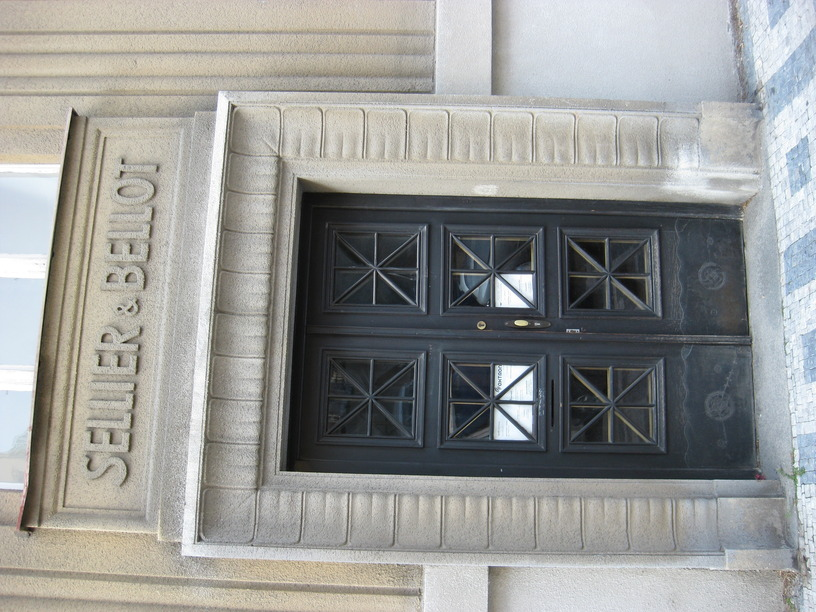
\includegraphics[width=4cm,angle=-90]{pictures/IMG_5955.JPG}}
			% }
			% \subfigure[] {
			% 	\fbox{\includegraphics[width=4cm,angle=-90]{pictures/IMG_5962.JPG}}
			% }
			% \subfigure[] {
			% 	\fbox{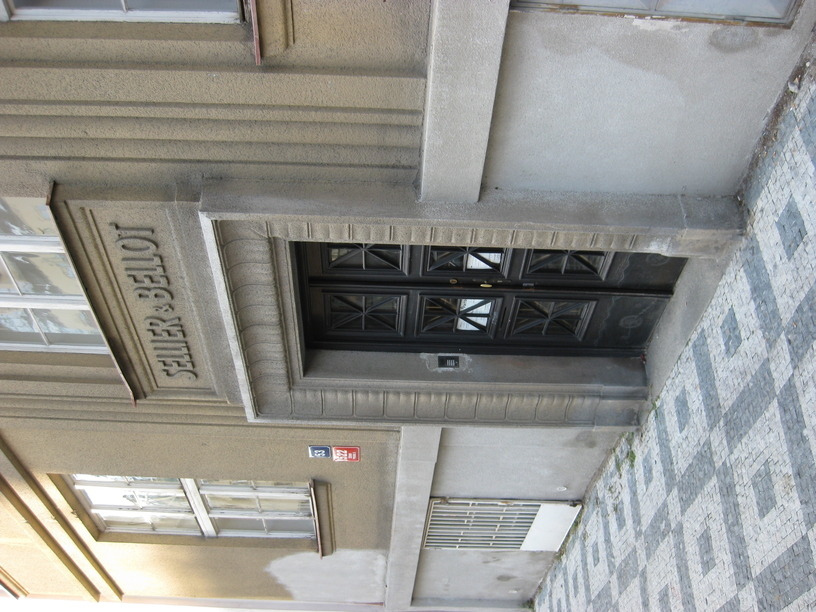
\includegraphics[width=4cm,angle=-90]{pictures/IMG_5965.JPG}}
			% }
			% \\
			% \subfigure[] {
			% 	\fbox{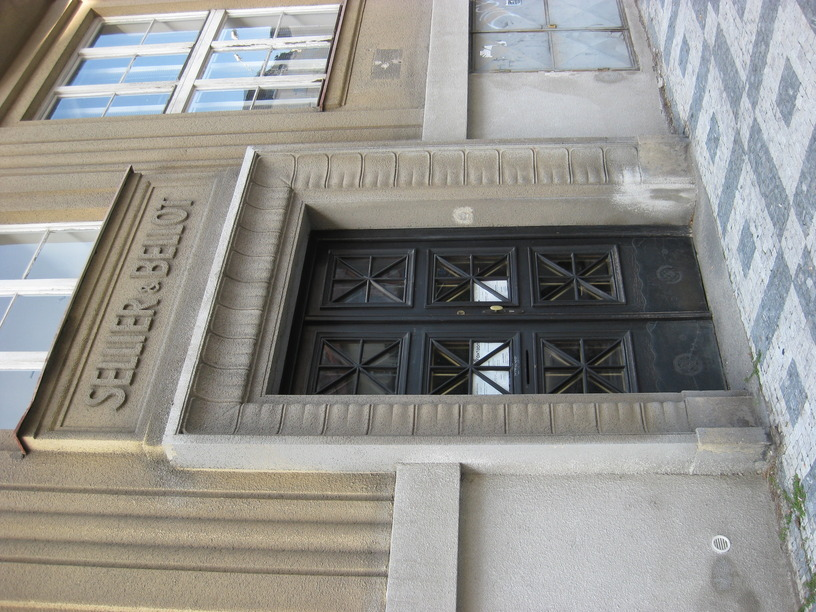
\includegraphics[width=4cm,angle=-90]{pictures/IMG_5957.JPG}}
			% }
			% \subfigure[] {
			% 	\fbox{\includegraphics[width=4cm,angle=-90]{pictures/IMG_5954.JPG}}
			%	\label{fig:i0}
			% }
			% \subfigure[] {
			% 	\fbox{\includegraphics[width=4cm,angle=-90]{pictures/IMG_5961.JPG}}
			%	\label{fig:i1}
			% }
			% \subfigure[] {
			% 	\fbox{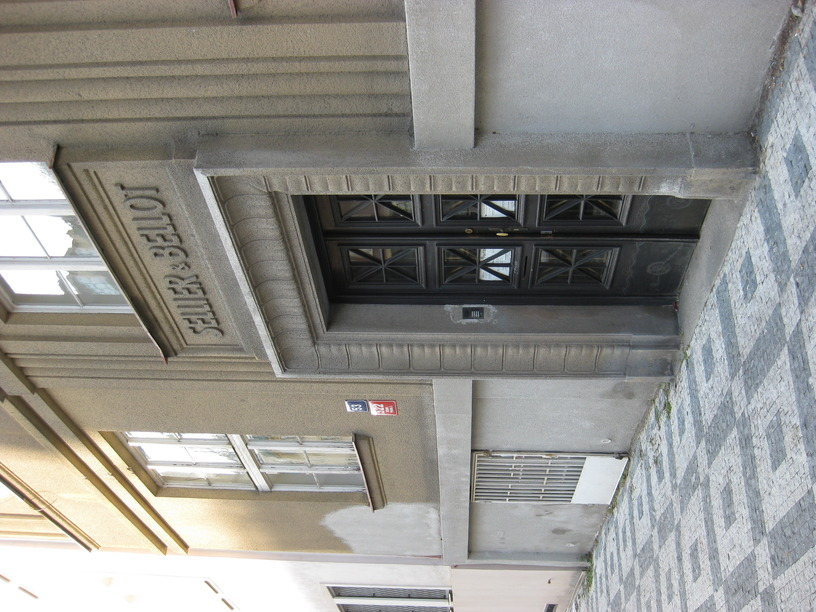
\includegraphics[width=4cm,angle=-90]{pictures/IMG_5964.JPG}}
			% }
			% \\
			% \subfigure[] {
			% 	\fbox{\includegraphics[width=4cm,angle=-90]{pictures/IMG_5956.JPG}}
			% }
			% \subfigure[] {
			% 	\fbox{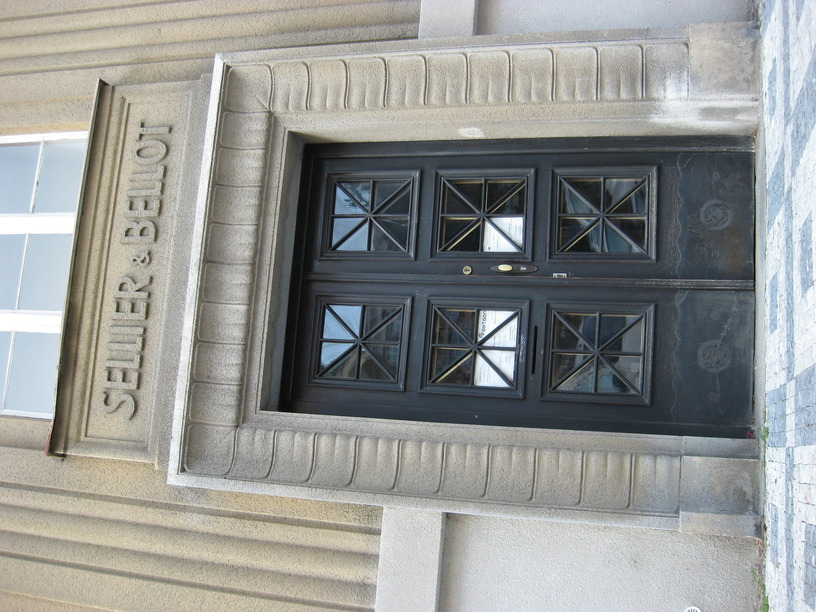
\includegraphics[width=4cm,angle=-90]{pictures/IMG_5953.JPG}}
			% }
			% \subfigure[] {
			% 	\fbox{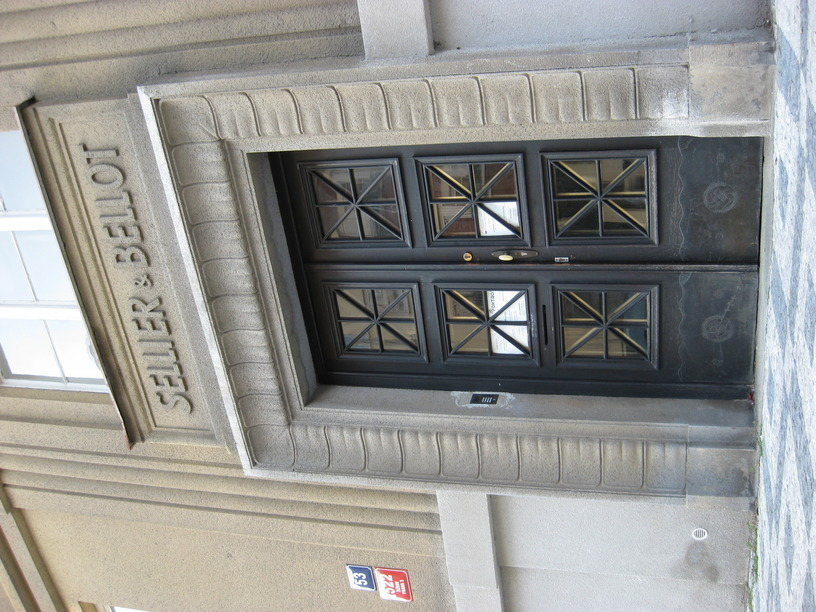
\includegraphics[width=4cm,angle=-90]{pictures/IMG_5960.JPG}}
			% }
			% \subfigure[] {
			% 	\fbox{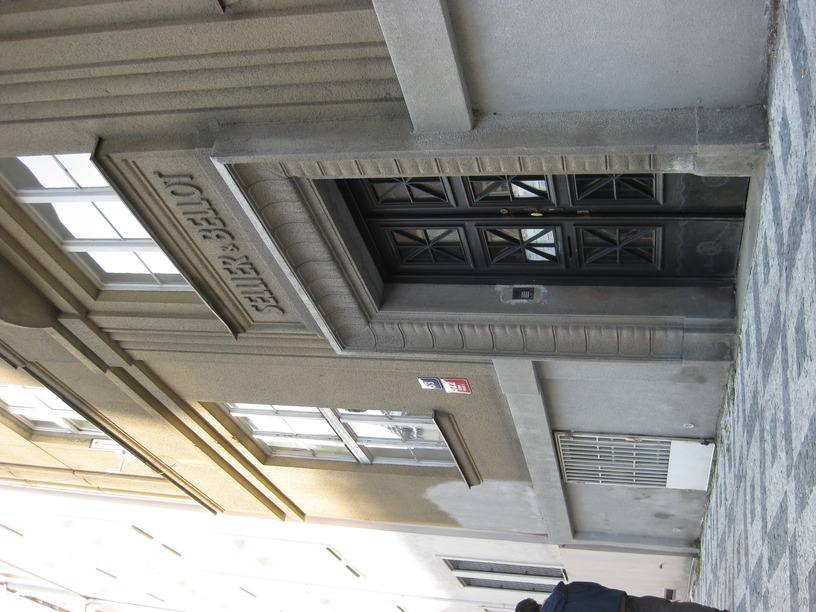
\includegraphics[width=4cm,angle=-90]{pictures/IMG_5963.JPG}}
			% }
		\caption{Nasnímané snímky, které byly použity pro rekonstrukci}
		\label{fig:inputPictures}
	\end{figure}

	\begin{figure}[htb]
		\centering
		\fbox{\includegraphics[width=16cm,angle=-90]{pictures/linear/IMG_5959.JPG}}
		\caption{Fotografie \ref{fig:firstInputImage} po odstranění radiálního zkreslení}
		\label{fig:linearizedPictureExample}
	\end{figure}

	\begin{figure}[htb]
			\centering
			\subfigure[] {
				\fbox{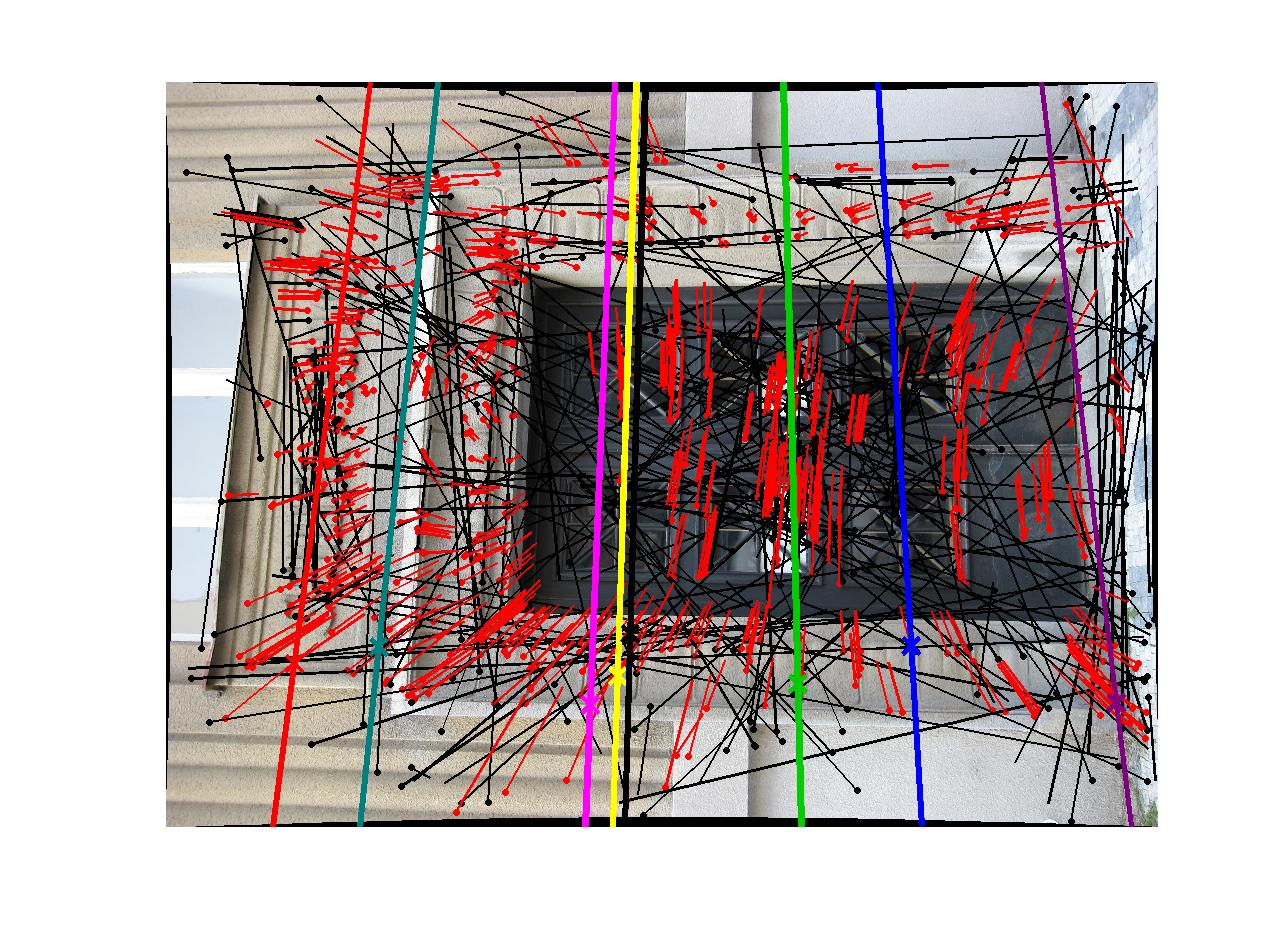
\includegraphics[width=8cm,angle=-90,clip=true,trim=165px 105px 110px 80px]{pictures/matches-left-with_epipolar_lines.jpg}}
			}
			\subfigure[] {
				\fbox{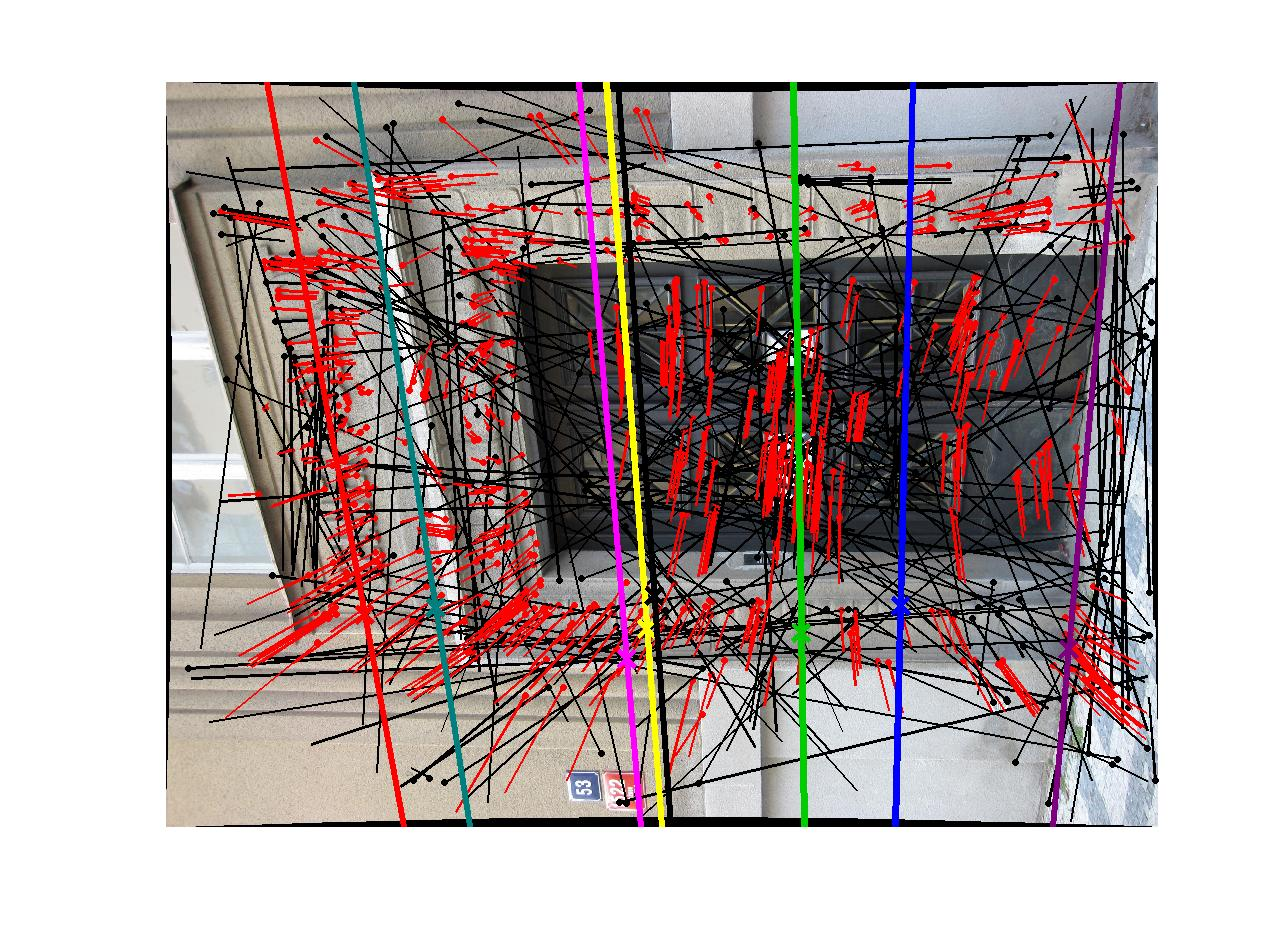
\includegraphics[width=8cm,angle=-90,clip=true,trim=165px 105px 110px 80px]{pictures/matches-right-with_epipolar_lines.jpg}}
			}
		\caption{Pár fotografií (\ref{fig:i0} a \ref{fig:i1}) se zobrazenými korespondencemi: červeně korespondence odpovídající
			epipolární geometrii, černě chybné. Pro vybrané body (označené křížky) jsou stejnými barvami znázorněny vzájemně si
			odpovídající epipoláry}
		\label{fig:pairWithEpipolars}
	\end{figure}

\section{Zhodnocení}

% FIXME: jak zahrnout bibliography.bib do repozitare? .. zkopirovat?

% Reference

	% FIXME:
	%	- zkontrolovat format oproti webu, zvolit vhodny .bst soubor
	%	- doplnit (?), aktualizovat odkazy a data

%\bibliographystyle{plain_cz}
\bibliographystyle{czechiso}
\bibliography{bibliography}

\end{document}

